    \documentclass{article}
\usepackage[utf8]{inputenc}
\usepackage{pgfplots}
\usepackage[utf8]{inputenc}
\usepackage[shortlabels]{enumitem}
\usepackage{amsmath} 
\usepackage{gensymb}
\usepackage{geometry}
\usepackage{listings}
\usepackage{xcolor}
\usepackage{pgfplots}
\usepackage{pgfplotstable}
\pgfplotsset{compat=1.7}
\usepackage{tikz}
\geometry{
 a4paper,
 total={170mm,257mm},
 left=20mm,
 top=20mm,
}
\title{Assignment: Two-variable Statistics}
\author{Andy Yan}
\date{September 2022}

\begin{document}

\maketitle
\textbf{Pg 210 Q8}
\section{Data}
A manufacturing company keeps records of its overall annual production and its number of employees. Data for a ten-year period are shown below. 
\begin{center}
\def\arraystretch{1}
{\setlength{\tabcolsep}{3em}
\begin{tabular}{| c | c | c |} 
 \hline
   Year & Number of Employees & Production (000)\\ 
 \hline
1992    & 158 & 75\\
 \hline
1993	& 165 & 81\\
 \hline
1994	& 172 & 84\\
 \hline
1995	& 148 & 68\\
 \hline
1996	& 130 & 58\\
 \hline
1997	& 120 & 51\\
 \hline
1998	& 98 & 50\\
 \hline
1999	& 105 & 57\\
 \hline
2000	& 110 & 62\\
 \hline
2001	& 120 & 70\\
  \hline
\end{tabular}}
\end{center}

\section{Scatter Plot}
\begin{center}
\begin{tikzpicture}
  \pgfplotsset{
      scale only axis,
  }
  \begin{axis}[
    xlabel=Number of Employees,
    ylabel=Production (000),
    xmin = 90,xmax = 180,
    ymin 45, ymax = 90,
    width=12cm,height=6cm,
  ]
    \addplot[only marks, mark=*]
    coordinates{ % plot 1 data set
      (158,75)
      (165,81)
      (172,84)
      (148,68)
      (130,58)
      (120,51)
      (98,50)
      (105,57)
      (110,62)
      (120,70)
      % more points...
    }; \label{plot_one}
    % plot 1 legend entry
    \addlegendimage{/pgfplots/refstyle=plot_one}
  \end{axis}
\end{tikzpicture}
\end{center}
a) 
To determine the behaviour of the graph, we must find the correlation coefficient (Pearson's r).
\[r = \frac{\sum (x - \overline x)(y - \overline y)}{\sqrt{\sum (x-\overline x)^2}\sqrt{\sum (y-\overline y)^2}} \approx \frac{278.49}{26.41\cdot11.97} \approx 0.88\]
Since r belongs in the range \(\frac{2}{3} \leq r < 1\), this scatter plot graph has a \textbf{strong positive linear correlation}.
\\\\
b) \textbf{1994-1995}
\\\\
c) The scatter plot does suggest that there is a hidden variable in play. We can see this when the company has 120 employees for two different, yet, the production differs. This could be due to worker efficiency and company management. We can assume that the company improved these factors since 1997 and that's why the production value is higher in 2001. The layoffs could suggest the company went under changes which shows us the temporary decline following it. However, we can see that the production starts improving as the company starts to regain employees.
\\\\
\section{Time-Series Graph (Productivity vs Year)}
d)
\begin{center}
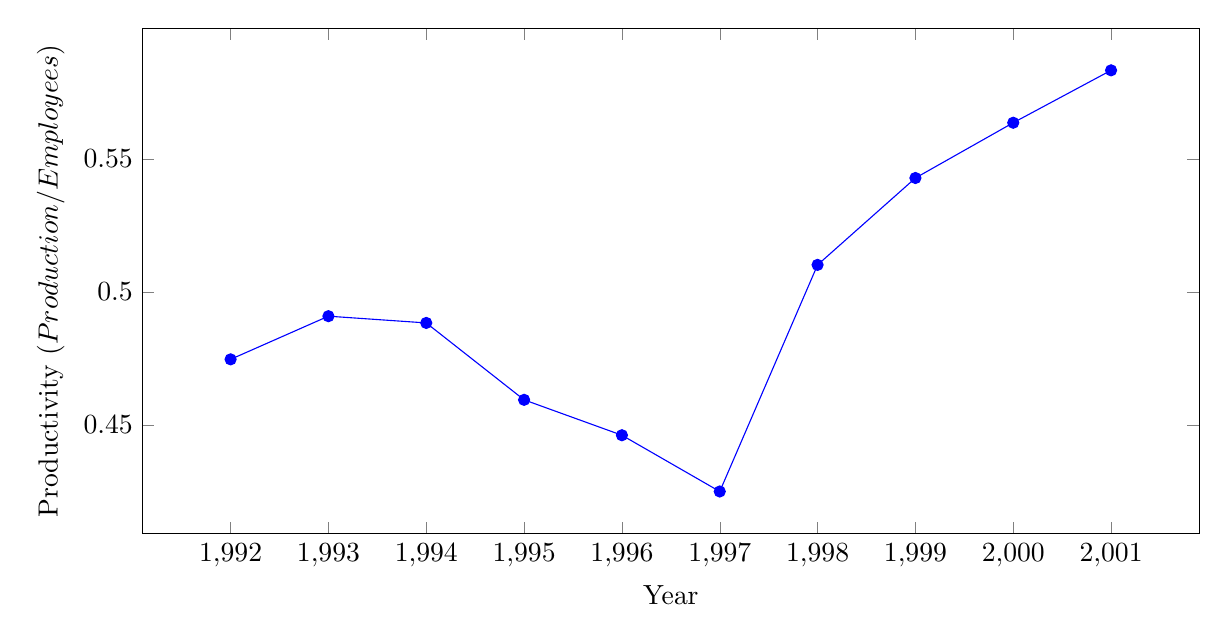
\begin{tikzpicture}
\begin{axis}[
	xlabel=Year,
	ylabel=Productivity (\({Production}/{Employees}\)),
	width=15cm,height=8cm,
    legend style={at={(0.0,.91)},anchor=west}
    ]

% Add values and attributes for the first plot
\addplot[color=blue,mark=*] coordinates {
      (1992,75/158)
      (1993,81/165)
      (1994,84/172)
      (1995,68/148)
      (1996,58/130)
      (1997,51/120)
      (1998,50/98)
      (1999,57/105)
      (2000,62/110)
      (2001,70/120)
};
\end{axis}
\end{tikzpicture}
\end{center}
e)
\[y=ax+b \]
\[a = \frac{n(\sum xy)-(\sum x)(\sum y)}{n(\sum x^2) - (\sum x)^2} = \frac{10(89492)-(1326)(656)}{10(182106)-(1326)^2} = \frac{3133}{7848} \approx 0.399\]
\[ b = \overline y - a\overline x\]
\[b = \frac{656}{10} - \frac{3133}{7848}\cdot\frac{1326}{10} \approx 12.665 \]
After solving for \(a\) and \(b\), we can write the equation for the line of best fit as:
\[y = 0.399x + 12.665\]
\begin{center}
\begin{tikzpicture}
  \pgfplotsset{
      scale only axis,
  }
  \begin{axis}[
    xlabel=Number of Employees,
    ylabel=Production (000),
    xmin = 90,xmax = 180,
    ymin 45, ymax = 90,
    width=12cm,height=6cm,
  ]
    
    
    \addplot[only marks, mark=*]
    coordinates{ % plot 1 data set
      (158,75)
      (165,81)
      (172,84)
      (148,68)
      (130,58)
      (120,51)
      (98,50)
      (105,57)
      (110,62)
      (120,70)
      % more points...
    }; \label{plot_one}
    
    \addplot[domain = 90:180,
        samples=100, 
        color=red,] {(3133/7848)*x + (656/10 - 4154358/78480)};
    
    % plot 1 legend entry
    \addlegendimage{/pgfplots/refstyle=plot_one}
  \end{axis}
\end{tikzpicture}
\end{center}
f) This system was implemented in 1997 as we can see in our time-series graph that it switches from decreasing to increase after 1997.

\end{document}
